\section{Cheat Sheet}

\subsection{Roots}

\begin{align*}
    \sqrt[n]{a}\cdot\sqrt[n]{b} & = \sqrt[n]{a\cdot b} \\
    \frac{\sqrt[n]{a}}{\sqrt[n]{b}} & = \sqrt[n]{\frac{a}{b}} \\
    (\sqrt[n]{a})^m & = \sqrt[n]{a^m} \\
    \sqrt[m]{\sqrt[n]{a}} & = \sqrt[m\cdot n]{a}
\end{align*}

\subsection{Logarithm}

\begin{align*}
    \log_n(a\cdot b) & = \log_n(a) + \log_N(b) \\
    \log_n(a\div b) & = \log_n(a) - \log_N(b) \\
    \log_n(a^b) & = b \cdot \log_n(a)
\end{align*}

\subsection{Trigonometry}

\begin{align*}
    \tan\theta & = \frac{\sin\theta}{\cos\theta} \\
    \sin -\theta & = -\sin\theta\text{ (cos same)} \\
    \sin 2\theta & = 2\sin\theta\cos\theta \\
    \cos 2\theta & = 2\cos^2\theta - \sin^2\theta = 2\cos^2\theta - 1 = 1 - 2\sin^2\theta \\
    \sin(\alpha \pm \beta) & = \sin\alpha\cos\beta\pm\cos\alpha\sin\beta \\
    \cos(\alpha\pm\beta) & = \cos\alpha\cos\beta \mp \sin\alpha\sin\beta
\end{align*}

\subsection{Binomial Coefficient}
\begin{align*}
	\binom{n}{k} = \frac{n!}{k!(n-k)!}
\end{align*}

\subsection{Determinant}
\makebox[\columnwidth]{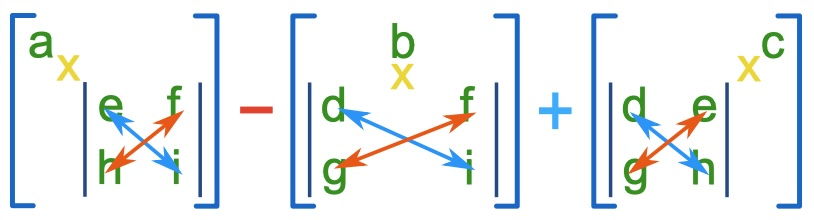
\includegraphics[width=0.5\columnwidth]{images/determinant}}

\begin{align*}
	\det
	\begin{bmatrix}
		a & b \\
		c & d
	\end{bmatrix}
	=
	ad-bc
\end{align*}
\begin{align*}
	\det
	\begin{bmatrix}
		a & b & c \\
		d & e & f \\
		g & h & i
	\end{bmatrix}
	=
	a(ei-fh)-b(di-fg)+c(dh-eg)
\end{align*}

\makebox[\columnwidth]{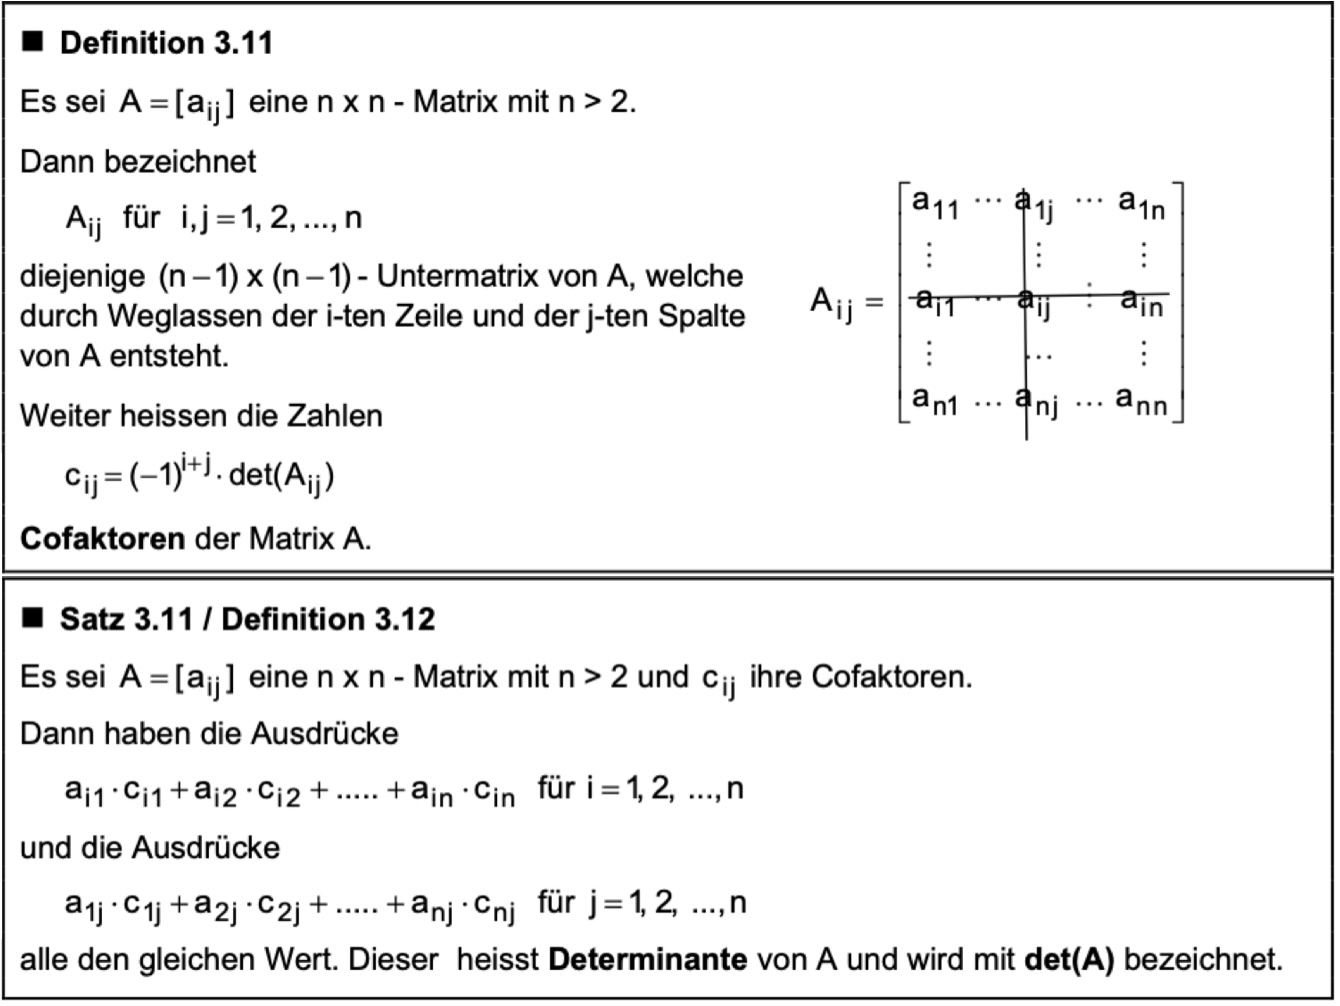
\includegraphics[width=\columnwidth]{images/determinant2}}

\subsection{Derivatives}
\begin{tabular}{r|l}
    $f(x)$                & $\frac{df}{dx}$                 \\
    \hline
    $\sinh(x)$            & $\cosh(x)$                      \\
    $\cosh(x)$            & $\sinh(x)$                      \\
    $\mathrm{arcsinh}(x)$ & $1 \div \sqrt{x^2+1}$           \\
    $\mathrm{arccosh}(x)$ & $1 \div \sqrt{x^2 - 1}$ ($1<x$) \\
    $\tan(x)$             & $\cos^{-2}(x)$                  \\
    $\log(x)$             & $x^{-1}$
\end{tabular}

\subsection{Integrals}
\begin{tabular}[h]{rl}
    $\int x^n\ dx$               & $= \frac{1}{n+1}x^{n+1} + C$             \\
    $\int \frac{1}{x}\ dx$       & $= \ln |x| + C$                          \\
    $\int \frac{1}{ax + b}\ dx$  & = $\frac{1}{a} \ln |ax+b| + C$           \\
    $\int \frac{1}{(x+a)^2}\ dx$ & $= -\frac{1}{x+a} + C$                   \\
    $\int \frac{1}{1 + x^2}$     & $= \tan^{-1} x + C$                      \\
    $\int \ln ax\ dx$            & $= x\ln ax - x + C$                      \\
    $\int e^{ax}\ dx$            & $= \frac{1}{a} e^{ax} + C$               \\
    $\int \sin(ax)\ dx$          & $= -\frac{1}{a}\cos(ax) + C$             \\
    $\int \sin^2(ax)\ dx$        & $= \frac{x}{2}-\frac{\sin(2ax)}{4a} + C$ \\
    $\int x\cos x\ dx$           & $= \cos x + x\sin x + C$                 \\
    $\int \sinh(ax)\ dx$         & $= a^{-1}\cosh{ax} + C$                  \\
    $\int \cosh(ax)\ dx$         & $= a^{-1}\sinh{ax} + C$                  \\
\end{tabular}

\subsection{Integration Techniques}

\subsubsection{Integration by Parts}
\begin{equation*}
    \int_a^b u(x)v'(x)\ dx = \left[ u(x)v(x) \right]_a^b-\int_a^bu'(x)v(x)\ dx
\end{equation*}

Or, with $u=u(x)$, $du=u'(x)\ dx$, $v=v(x)$ and $dv=v'(x)\ dx$:
\begin{equation*}
    \int u\ dv=uv - \int v\ du
\end{equation*}

\subsubsection{Substitution}
\begin{equation*}
    \int_a^b f(g(x))\cdot g'(x)\ dx = \int_{g(a)}^{g(b)}f(u)\ du
\end{equation*}

\subsubsection{Leibniz Integral Rule}
\begin{multline*}
    \frac{d}{dx}\left(\int_{a(x)}^{b(x)}f(x,t)\ dt\right)
    =
    \\
    f(x,b(x))\cdot\frac{d}{dx}b(x)
    -f(x,a(x))\cdot\frac{d}{dx}a(x)
    +\int_{a(x)}^{b(x)}\frac{\partial}{\partial x}f(x,t)\ dt
\end{multline*}
Special case where $a(x)=a=\mathrm{const.}$ and $b(x)=b=\mathrm{const.}$:
\begin{equation*}
    \frac{d}{dx}\left(\int_a^b f(x,t)\ dt\right)
    =\int_a^b\frac{\partial}{\partial x}f(x,t)\ dt
\end{equation*}

\subsection{Particular Solutions to Simple ODEs}

\begin{tabular}[h]{rcl}
    $f'(x)=\frac{c}{x}f(x)$ & $\Rightarrow$ & $f(x)=k_1y^c$                                             \\
    $f'(x)=x\cdot f(x)$     & $\Rightarrow$ & $f(x)=k_1e^{cx}$                                          \\
    $f''(x) = c\cdot f(x)$  & $\Rightarrow$ & $f(x) = k_1e^{\sqrt{c}x}+k_2e^{-\sqrt{c}x}$               \\
    $f''(x) = -c\cdot f(x)$ & $\Rightarrow$ & $f(x)=k_1\sin(\sqrt{c}x)+k_2\cos(\sqrt{c}x)$              \\
    $f'(x)+af(x) = b$       & $\Rightarrow$ & $f(x) = \left(f(0)-\frac{b}{a}\right)e^{-ax}+\frac{b}{a}$
\end{tabular}
